\chapter{Experiment 4: Bounded Classifier and Optimization Tuning}
\label{ch:v4}

\section{Frozen scope}

V4 uses exactly the V3 88-person inputs, delay moments, spectral controls, and
outer subject splits. No new EEG exclusion or transformation is introduced.
Before new outer outcomes are examined, 139 configurations are saved in
\code{protocol.json}. This bounds researcher degrees of freedom and makes the
reported tuning reproducible.

\section{Representation grid}

Seven unsupervised feature settings are crossed with 19 classifiers:

\begin{itemize}
  \item waveform TT terminal rank 8 or 16, channel rank 6;
  \item waveform Tucker channel/lag rank 4 or 6;
  \item 418 spectral controls with training-only selection of 16 or 32;
  \item TT16 concatenated with 418 spectral controls, followed by training-only
  selection of 32 combined features.
\end{itemize}

The fusion setting does not guarantee use of TT features. ANOVA selection can
choose mostly or entirely spectral variables. A fusion win is therefore evidence
for the complete representation-selection pipeline, not isolated proof of a
tensor contribution.

\section{Classifier grid}

The 19 settings are:

\begin{itemize}
  \item logistic regression with $C\in\{0.01,0.1,1\}$;
  \item RBF SVM with $C\in\{0.1,1,10\}$ and
  $\gamma\in\{\text{scale},0.01\}$ \citep{cortes1995svm};
  \item eight fixed XGBoost combinations spanning depth 1--3, learning rate
  0.03--0.1, 100--250 trees, minimum child weight 1--5, $L_2$ penalty 1--10,
  $L_1$ penalty 0--0.5, row subsampling 0.8--1.0, and column subsampling 0.8
  \citep{chen2016xgboost}; and
  \item two 200-tree random forests: depth 3/minimum leaf 3, or unrestricted
  depth/minimum leaf 5, with square-root feature sampling
  \citep{breiman2001rf}.
\end{itemize}

All pipelines standardize features, including tree models, for one consistent
persisted schema. Classifier fitting receives the weights in
Eq.~\ref{eq:class-weight}. XGBoost uses CPU histogram trees, multiclass soft
probabilities, fixed tree counts, and no test-driven early stopping.

\section{Stronger-regularized supervised TT}

Six additional supervised TT settings use channel rank 2 or 4, 4 or 8 filters,
head penalty 0.1 or 1, core anchor 0.1 or 1, and a fixed 500-iteration budget.
The altered objective replaces the weak $10^{-3}$ anchor from V3 with a much
stronger constraint toward the training-only unsupervised TT initialization.
Analytic gradients are numerically checked before benchmarking.

\section{Selection hierarchy}

For each outer fold, three-fold inner out-of-fold predictions rank all 139
configurations by balanced accuracy, then macro F1, then deterministic lower
complexity. The code saves ten outer entries:

\begin{itemize}
  \item one complete inner-selected pipeline (the primary endpoint);
  \item best inner-selected member of each of five classifier families; and
  \item best inner-selected member of each of four representation families.
\end{itemize}

These are not ten statistically independent fitted models; several named views
can reference the same fitted configuration. Per-family scores are secondary
comparisons and cannot replace the primary result after test inspection.

\section{Software execution}

The official \code{xgboost-cpu==3.2.0} package was installed into the existing
Python 3.10 user environment without upgrading dependencies, creating a virtual
environment, installing PyTorch, or enabling CUDA. The fitted XGBoost build
reports OpenMP enabled and CUDA disabled. Nested fitting took 316.3 seconds,
excluding installation and verification. Core estimators use scikit-learn's
pipeline interfaces \citep{pedregosa2011sklearn}.

\section{Results}

\begin{figure}[htbp]
\centering
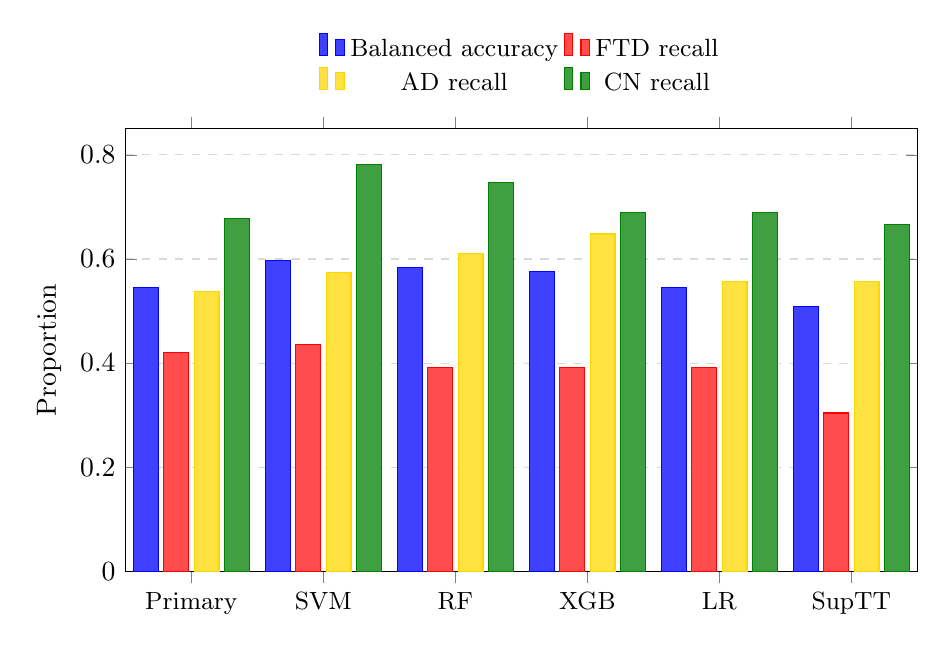
\begin{tikzpicture}
\begin{axis}[
  ybar,
  width=0.96\textwidth,
  height=72mm,
  bar width=9pt,
  ymin=0,ymax=0.85,
  ylabel={Proportion},
  symbolic x coords={Primary,SVM,RF,XGB,LR,SupTT},
  xtick=data,
  x tick label style={font=\small,rotate=0},
  ymajorgrids=true,
  grid style={dashed,gray!30},
  legend style={at={(0.5,1.23)},anchor=north,legend columns=2,draw=none,font=\small},
  enlarge x limits=0.10
]
\addplot[fill=Blue!75,draw=Blue] coordinates {(Primary,0.545) (SVM,0.597) (RF,0.583) (XGB,0.576) (LR,0.546) (SupTT,0.509)};
\addplot[fill=Red!70,draw=Red] coordinates {(Primary,0.420) (SVM,0.435) (RF,0.391) (XGB,0.391) (LR,0.391) (SupTT,0.304)};
\addplot[fill=Gold!75,draw=Gold] coordinates {(Primary,0.537) (SVM,0.574) (RF,0.611) (XGB,0.648) (LR,0.556) (SupTT,0.556)};
\addplot[fill=Green!75,draw=Green] coordinates {(Primary,0.678) (SVM,0.782) (RF,0.747) (XGB,0.690) (LR,0.690) (SupTT,0.667)};
\legend{Balanced accuracy,FTD recall,AD recall,CN recall}
\end{axis}
\end{tikzpicture}
\caption{V4 classifier-family balanced accuracy and diagnosis recall. SVM is the strongest observed family, while FTD recall remains the weakest class-specific measure.}
\label{fig:v4-classifier}
\end{figure}


The complete automatic-selection endpoint is 54.5\% mean balanced accuracy
(repeat SD 3.2 pp), ordinary accuracy 55.3\%, and macro F1 0.540. It improves
nominally by 2.5 percentage points over V3's 52.0\% primary endpoint on the same
inputs and outer splits, but adaptive reuse of the cohort prevents treating this
as independent confirmation.

The strongest observed classifier family is RBF SVM at 59.7\% mean balanced
accuracy (repeat SD 0.9 pp), ordinary accuracy 60.6\%, and macro F1 0.589.
Random forest reaches 58.3\%; XGBoost 57.6\%; logistic regression 54.6\%; and
stronger-regularized supervised TT 50.9\%. SVM is stronger than XGBoost in this
bounded comparison.

Representation-family results are TT/spectral fusion 59.1\% (SD 3.6 pp),
spectral 56.8\% (SD 1.2 pp), waveform Tucker 52.0\% (SD 2.3 pp), and waveform TT
46.8\% (SD 11.7 pp). The large TT repeat variability is a warning against
selecting a favorable repeat or fold.

\section{Optimization and verification}

Among 285 supervised optimization fits, 200 report convergence and 85 reach the
500-iteration limit. This is an optimization-status improvement over V3 but not
a predictive win. Verification passes all of the following:

\begin{itemize}
  \item 150 saved outer model entries replayed with matching scores;
  \item 60 training-only basis sets and 45 inner plus 15 outer splits checked;
  \item exact inner selections, scaler means, and class-weight totals reproduced;
  \item 23 XGBoost boosters exported and reloaded with matching outputs; and
  \item original primary and leftover array hashes unchanged.
\end{itemize}

